% Stock-Market Dynamics: A Graph-Based Cluster-Dynamics Model of S&P 500 Regimes
% Style adapted from the NuMat 2026 presentation
% "Graph-Based Cluster Dynamics of Irradiated Materials" (N.M. Ghoniem).
\documentclass[11pt,a4paper]{article}

\usepackage[margin=2.4cm]{geometry}
\usepackage{amsmath,amssymb}
\usepackage{graphicx}
\usepackage[font=small,labelfont=bf]{caption}
\setlength{\abovecaptionskip}{4pt}
\setlength{\belowcaptionskip}{4pt}
\setlength{\textfloatsep}{8pt}
\setlength{\floatsep}{6pt}
\renewcommand{\topfraction}{0.9}
\renewcommand{\bottomfraction}{0.9}
\renewcommand{\textfraction}{0.05}
\setcounter{totalnumber}{5}
\setcounter{topnumber}{5}
\usepackage{xcolor}
\usepackage{tikz}
\usetikzlibrary{arrows.meta,positioning,shapes,calc}
\usepackage{booktabs}
\usepackage{longtable}
\usepackage{tabularx}
\usepackage{sectsty}
\usepackage{fancyhdr}
\usepackage{helvet}
\renewcommand{\familydefault}{\sfdefault}

\definecolor{nmblue}{RGB}{0,51,153}
\definecolor{nmgray}{RGB}{90,90,90}

\usepackage[colorlinks=true,linkcolor=nmblue,citecolor=nmblue,urlcolor=nmblue]{hyperref}

\allsectionsfont{\color{nmblue}\sffamily\bfseries}
\subsectionfont{\color{nmblue!80!black}}

\pagestyle{fancy}
\fancyhf{}
\fancyfoot[L]{\footnotesize\textcolor{nmgray}{N.M. Ghoniem}}
\fancyfoot[C]{\footnotesize\textcolor{nmgray}{Stock-Market Dynamics: S\&P 500 Regime Clusters, 2000--2021}}
\fancyfoot[R]{\footnotesize\textcolor{nmgray}{\thepage}}
\renewcommand{\headrulewidth}{0pt}

\setlength{\parskip}{0.45em}
\setlength{\parindent}{0pt}

\begin{document}

% ---------------- Title block (presentation title-page style) ----------------
\begin{center}
\vspace*{0.5cm}
{\LARGE\bfseries\color{nmblue} Stock-Market Dynamics:\\[0.3em]
A Graph-Based Cluster-Dynamics Model\\[0.3em] of S\&P 500 Market Regimes, 2000--2021}
\vspace{0.4cm}

{\large Nasr M. Ghoniem}

{\normalsize Department of Mechanical \& Aerospace Engineering\\
University of California, Los Angeles}
\vspace{0.3cm}

{\normalsize\textcolor{nmgray}{Technical documentation, September 2026}}
\vspace{0.4cm}

{\small\textcolor{nmgray}{Adapted from the graph-based cluster-dynamics framework
(RadCluster): the market-regime bin is a \emph{cluster}, the stocks are the
migrating particles, and the ``reactions'' are regime drift, herding flows,
and index entry/exit.}}
\end{center}
\vspace{0.6cm}

\tableofcontents
\newpage

% ---------------- Abstract ----------------
\begin{abstract}
\noindent We present a cluster-dynamics prototype that ports the RadCluster
reaction--advection framework to the cross-sectional distribution of S\&P~500
stocks across market regimes.  The state is the 15-bin regime distribution
$\mathbf{c}(t)\in\mathbb{R}^{15}$ (5 absolute momentum bins $\times$ 3
volatility terciles).  Four reaction kernels act on it: (i) a
\textbf{measured} Markov drift $\mathbf{T}$; (ii) \textbf{market advection},
a rigid translation of the distribution along the momentum axis driven by
the measured cross-sectional window-delta
$M_{\mathrm{cs}}(t)=r(t)-r(t-12)$; (iii) \textbf{autocatalytic herding}, a
bilinear flux toward above-average-momentum bins with signed rate
$h_{\mathrm{eff}}=h_1(w-\ell)$; (iv) a \textbf{spike-persistence damper}
that impedes extreme-bin outflow on driver-sign reversal, modeling the
unresolvable within-bin tail depth.  Two out-of-sample hindcasts
conditioned on the realized market move --- the 2020--21 COVID recovery
and the 2008--09 financial crisis --- reproduce the observed concentration
spikes ($0.515$ vs.\ $0.546$ actual top-bin peak, 2021; $0.994$ vs.\
$0.978$ actual bottom-bin peak, 2008) and their post-peak decay
($+1$-month: $0.418$ vs.\ $0.406$, 2021; $0.988$ vs.\ $0.966$, 2008) with
full-distribution RMSE $0.0914$ and $0.1037$.  The advection kernel is the
spike generator; herding is an amplifier; the persistence damper is the
decay-rate kernel.  All inputs are labeled measured / mechanical /
calibrated / assumed.  The hindcast is conditional on realized $M_{\mathrm{cs}}$
(exogenous forcing), not a lookahead-free forecast.
\end{abstract}

% ---------------- 1. Introduction ----------------
\section{Introduction}
This document describes a stock-market prototype built by reusing the
graph-based modeling approach of RadCluster: the market is partitioned into
discrete regime classes (vertices), and every capital-migration process is an
admissible transition (edge) carrying a rate kernel.  The state is integrated
as a system of ordinary differential equations over 2000--2021, and validated
against two hindcast episodes: the 2020--21 COVID concentration and the
2008--09 financial-crisis drawdown.

In the language of the cluster-dynamics framework, the market-regime bin is
a \emph{cluster}: each stock belongs to a cluster $R_{mv}$ labeled by its
momentum bin $m=0,\dots,4$ and volatility bin $v=0,1,2$, the direct analog of
the cluster size in the materials formulation.  The stocks are the migrating
particles; $\mathbf{c}(t)\in\mathbb{R}^{15}$ is the distribution of index
stocks across the 15 regime clusters.  The bins use \emph{absolute}
thresholds, not cross-sectional ranks: momentum is the trailing 12-minus-1
month return on adjusted close in the bands
$<0\%$, $0$--$15\%$, $15$--$30\%$, $30$--$60\%$, $>60\%$;
volatility is the trailing-60-trading-day annualized standard deviation of
daily log returns in the terciles $<20\%$, $20$--$32\%$, $>32\%$.
Absolute bins are essential: quintile ranks would freeze every marginal at
$20\%$ by construction and the distribution could never concentrate, which
is the phenomenon under study.

Three edge classes act on the graph, plus the forcing and the rev.~3
persistence damper:
\begin{itemize}
  \item \textbf{Drift} --- the measured month-to-month Markov transition
    matrix $\mathbf{T}$: momentum builds or decays and volatility shifts, so
    stocks wander between adjacent regime bins.  A single stationary
    $\mathbf{T}$ is estimated per episode on pre-episode data, made
    concentration-sticky via $\mathbf{T}_{\mathrm{eff}}$ (Sec.~2).
  \item \textbf{Market advection} --- the measured window-delta
    $M_{\mathrm{cs}}(t)$ rigidly translates the distribution along the
    momentum axis; the unbounded extreme bins accumulate mass and generate
    spikes (Sec.~2).
  \item \textbf{Herding} --- the bilinear winner-chasing flux with the
    autocatalytic rate $h_{\mathrm{eff}}=h_1(w-\ell)$, the market analog of
    the assortativity/mating term: capital flows toward recent winners (or
    away from losers in a crash), the candidate amplifier of concentration
    episodes.  $h_1=0$ is the drift-only null.
  \item \textbf{Spike persistence (rev.~3)} --- damps the extreme-bin outflow
    when the market reverses out of a spike, modeling the within-bin tail
    depth the 15-bin state cannot resolve (Sec.~2, Eq.~\eqref{eq:damp}).
  \item \textbf{Source/sink} --- index additions (IPOs, promotions) and
    removals (delistings, acquisitions), measured but tiny.
\end{itemize}
The forecasting objective is the \emph{future regime distribution}: what
fraction of the market sits in each bin next month, and in particular its
\emph{concentration} --- whether capital crowds into winner bins or disperses.
Individual stock prices are not predicted.

Two hindcast cases are carried: \textbf{Case~1}, the 2020--21 COVID episode
(a recovery-driven concentration: $55\%$ of stocks above $60\%$ twelve-month
return in March~2021, measured off the crash bottom); and \textbf{Case~2},
the 2008--09 financial crisis (a drawdown: $98\%$ of stocks in the loser bin
at the March~2009 peak).  Both are run out-of-sample from pre-episode calibration.

% ---------------- 1b. Related work ----------------
\section{Related work}
The momentum leg of the model rests on the cross-sectional momentum
literature: Jegadeesh and Titman~\cite{jegadeesh1993} documented that buying
recent winners and selling recent losers earns abnormal returns over 3--12
month horizons, the empirical basis for treating trailing return as a regime
coordinate.  Fama and French~\cite{fama1993} systematized common risk factors
in equity returns; volatility as the second regime axis follows the same
risk-factor logic.

The herding term belongs to the econophysics tradition of imitation-driven
market models.  Cont and Bouchaud~\cite{cont2000} showed that random
percolation-like herding generates the heavy-tailed return distributions seen
in real markets from purely imitative agents.  Lux and
Marchesi~\cite{lux1999} built a stochastic multi-agent model in which
chartist--fundamentalist switching produces scaling and volatility
clustering; the herding flux here is the mean-field, cluster-level
counterpart of their switching dynamics.  At the behavioral level, Barberis,
Shleifer and Vishny~\cite{barberis1998} modeled investor sentiment as
conservatism plus representativeness, giving under- and over-reaction ---
the psychological microfoundation for winner-chasing flows.

Regime dependence of the drift follows Hamilton~\cite{hamilton1989}, whose
Markov-switching model of nonstationary economic time series is the direct
antecedent of the VIX-split transition pair
$(\mathbf{T}_{\mathrm{calm}},\mathbf{T}_{\mathrm{stress}})$ used here.

What is new here is the combination: a forward-time cluster-dynamics ODE
framework ported from irradiated-materials modeling, with the market regime
as the cluster, stocks as the migrating particles, a bilinear herding
``reaction'' as the tested concentration mechanism, and two out-of-sample
hindcast episodes (2020--21, 2008--09) on measured S\&P~500 data.

% ---------------- 2. Model formulation ----------------
\section{Model formulation}
\subsection{State, clusters and regimes}
The state is $\mathbf{c}(t)\in\mathbb{R}^{15}$ with
$c_{k}(t)$ the fraction of S\&P~500 constituents in regime bin
$k=3m+v$, $m=0,\dots,4$ the momentum bin, $v=0,1,2$ the volatility bin.
Momentum for stock $i$ at month-end $t$ is the 12-minus-1 month total return
on adjusted close (measured); volatility is the annualized standard
deviation of daily log returns over the trailing 60 trading days (measured).
Bins are absolute (Sec.~1), recomputed from the measured features each
month; the panel runs 2000-12 through 2022-01 (253 months, 106{,}885
stock-months; the constituent count grows 343$\to$486 over the window).

\subsection{Master equation in matrix form}
The dynamics take the compact form
\begin{equation}
  \frac{d\mathbf{c}}{dt} \;=\; \mathbf{P}(t) + \mathbf{S}\,\mathbf{J}(\mathbf{c})
  \;-\; \mathbf{D}(t)\,\mathbf{c},
  \label{eq:master}
\end{equation}
with the pieces identified as follows.
\begin{itemize}
  \item \textbf{Source vector:} $\mathbf{P}(t)\in\mathbb{R}^{15}$ ---
    index additions $s(t)$ enter uniformly across bins (measured mean
    $8\times10^{-4}$/month); removals are proportional at rate $d(t)$
    (measured $\approx 0$).  Net effect on the distribution is negligible;
    the state is renormalized each step.
  \item \textbf{Stoichiometry and flux:} the drift is the linear part
    $\mathbf{T}_{\mathrm{eff}}^{\!\top}\mathbf{c}$ with $\mathbf{T}$ the
    measured monthly Markov transition matrix (discrete-time form).
    The herding flux is the bilinear term
    \begin{equation}
      H_k(\mathbf{c}) \;=\; c_k\,\frac{q_k-\bar q(\mathbf{c})}{4},
      \qquad
      \bar q(\mathbf{c})=\sum_j c_j q_j,
      \label{eq:herding}
    \end{equation}
    where $q_k\in\{0,\dots,4\}$ is the momentum bin of cluster $k$.
    $H$ is zero-sum by construction ($\sum_k H_k=0$): it moves mass from
    below-average-momentum bins to above-average-momentum bins, the
    market counterpart of the assortative-mating flux.
  \item \textbf{Market advection (the spike generator).} When the market's
    trailing twelve-month return shifts by $M$ in a month, every stock's
    momentum shifts by $\sim\!M$ in return space --- a rigid translation
    of the distribution along the momentum axis, driven mechanically by
    window rollover (the month entering the 12-month window replaces the
    month dropping out).  The driver
    \begin{equation}
      M_{\mathrm{cs}}(t) \;=\; r(t) - r(t-12)
      \label{eq:mcs}
    \end{equation}
    is the \emph{synchronized change in twelve-month momentum}, measured
    cross-sectionally (equal-weighted over all index stocks).
    March~2021: $M_{\mathrm{cs}}=+0.256$; October~2008:
    $M_{\mathrm{cs}}=-0.256$.  The donor-cell update moves fraction
    $f=\kappa|M_{\mathrm{cs}}|/w_{\mathrm{eff}}$ of each momentum bin to
    the next ($\kappa=1.0$ mechanical, $w_{\mathrm{eff}}=0.15$ assumed);
    the unbounded extreme bins ($<0\%$, $>60\%$) reflect and accumulate
    mass --- this is what generates spikes.
  \item \textbf{Autocatalytic herding (the amplifier).} The herding rate
    grows with the winner concentration itself:
    \begin{equation}
      h_{\mathrm{eff}} \;=\; h_0 + h_1\,(w - \ell),
      \label{eq:autoherd}
    \end{equation}
    with $w,\ell$ the top/bottom momentum shares.  The signed form is
    deliberate: in a crash ($\ell\gg w$) it drives mass toward losers
    (panic selling); in a melt-up ($w\gg\ell$) toward winners (FOMO).
    It is symmetric by construction --- the data decide the sign.
  \item \textbf{Sticky drift (the persistence kernel).}
    $\mathbf{T}_{\mathrm{eff}}=(1-\lambda)\mathbf{T}+\lambda\mathbf{I}$,
    with $\lambda=\min[\lambda_1\max(w,\ell),0.9]$.  When the distribution
    piles into an extreme bin, the drift freezes toward identity and the
    spike persists; at low concentration ordinary drift applies.
\end{itemize}
In discrete monthly time the integrated form is
\begin{equation}
  \mathbf{c}(t{+}1) \;=\; \mathbf{T}_{\mathrm{eff}}^{\!\top}\mathbf{c}(t)
  + \mathrm{advect}(\mathbf{c}(t), M_{\mathrm{cs}})
  + h_{\mathrm{eff}}\,\mathbf{H}(\mathbf{c}(t)) + \mathbf{s} - d\,\mathbf{c}(t),
  \label{eq:discrete}
\end{equation}
renormalized to sum 1 each step.  The transition $t_0\to t_1$ uses the
\emph{destination-month} driver $M_{\mathrm{cs}}(t_1)$, because the window
rollover defining $M(t_1)$ is what moves stocks between bins during that
month --- making the hindcast \emph{conditional} on the realized market
move (exogenous forcing), not a lookahead-free forecast.

\subsection{Why these vertices and edges}
Momentum and volatility are the two measured features along which equity
crowding episodes visibly separate: in every historical concentration event
the winner cohort is simultaneously high-momentum and elevated-volatility,
while the loser cohort pools in the low-momentum bins.  Absolute bins keep
the cluster semantics of the materials framework (a cluster \emph{size} is a
fixed state, not a rank).  Drift is measured rather than modeled because the
month-to-month migration statistics are directly observable; herding is the
single free mechanism parameter $h_1$ because winner-chasing is the
hypothesis under test, and isolating it as one bilinear term keeps the null
($h_1=0$) sharp.  Advection carries no free parameter ($\kappa=1$ is the
mechanical identity: a percentage point is a percentage point) --- it is the
distribution-level consequence of twelve-month window rollover, measured
through $M_{\mathrm{cs}}$.

% ---------------- 3. Market-dynamics graph ----------------
\section{Market-dynamics graph}
\label{sec:rag}
The reaction graph below is drawn from the model specification: every vertex
is a real state variable $c_k$, every edge a real term of the right-hand
side of Eq.~\eqref{eq:discrete}.  Vertices are the 15 regime clusters
$R_{mv}$ on the momentum ($m$) $\times$ volatility ($v$) lattice; blue edges
are the dominant measured drift transitions ($T_{ij}>0.08$); the red arrow is
the herding ratchet, which carries mass rightward toward the winner column
at rate $h$; index entry/exit attach as source/sink.

\begin{figure}[htbp]
\centering
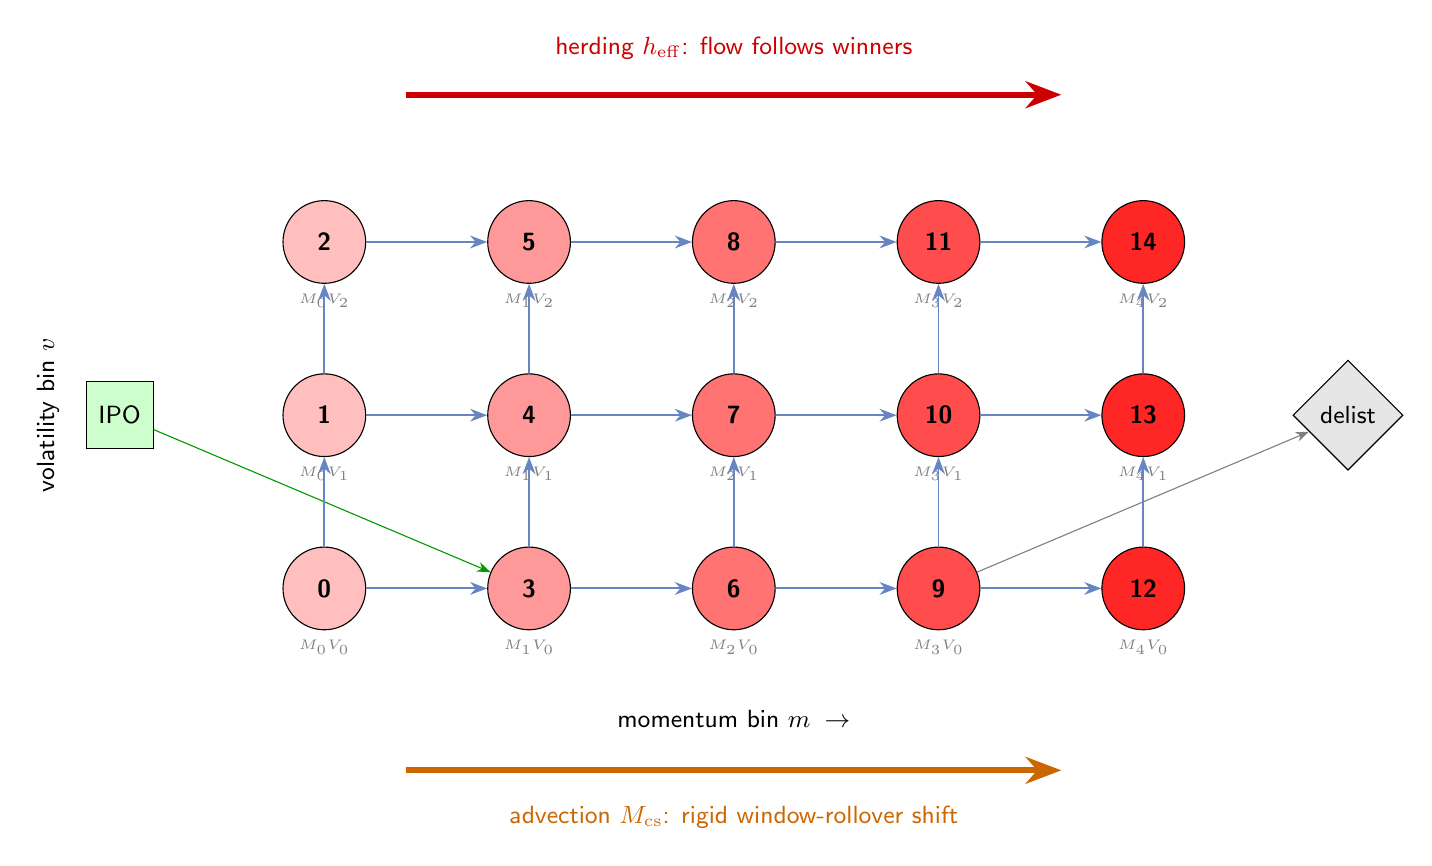
\begin{tikzpicture}[x=2.6cm,y=2.2cm,
  rv/.style={circle,draw,minimum size=1.05cm,inner sep=1pt,font=\small\bfseries},
  src/.style={rectangle,draw,minimum size=0.85cm,font=\small},
  sink/.style={diamond,draw,minimum size=0.85cm,font=\small}]
  % vertices: momentum 0..4 (x), volatility 0..2 (y)
  \foreach \m in {0,...,4} {
    \foreach \v in {0,...,2} {
      \pgfmathtruncatemacro{\b}{\m*3+\v}
      \pgfmathsetmacro{\shade}{25+15*\m}
      \node[rv,fill=red!\shade!white] (R\b) at (\m,\v) {\b};
      \node[font=\tiny,gray] at (\m,\v-0.34) {$M_{\m}V_{\v}$};
    }
  }
  % source / sink
  \node[src,fill=green!20] (SRC) at (-1,1) {IPO};
  \node[sink,fill=gray!20] (SNK) at (5,1) {delist};
  \draw[-{Stealth},green!60!black] (SRC) -- (R3);
  \draw[-{Stealth},gray] (R9) -- (SNK);
  % dominant drift edges (measured T_ij > 0.08, schematic adjacency)
  \foreach \a/\b in {0/3,1/4,2/5,3/6,4/7,5/8,6/9,7/10,8/11,9/12,10/13,11/14,
                     0/1,3/4,6/7,9/10,12/13,1/2,4/5,7/8,10/11,13/14} {
    \draw[-{Stealth},nmblue!60,line width=0.7pt] (R\a) -- (R\b);
  }
  % herding ratchet annotation (above the lattice, clear of nodes)
  \draw[-{Stealth},red!80!black,line width=2.2pt] (0.4,2.85) -- (3.6,2.85);
  \node[font=\small,red!80!black] at (2.0,3.12) {herding $h_{\mathrm{eff}}$: flow follows winners};
  % market-advection annotation (below the lattice)
  \draw[-{Stealth},orange!80!black,line width=2.2pt] (0.4,-1.05) -- (3.6,-1.05);
  \node[font=\small,orange!80!black] at (2.0,-1.32) {advection $M_{\mathrm{cs}}$: rigid window-rollover shift};
  % axes
  \node[font=\small] at (2,-0.75) {momentum bin $m\;\rightarrow$};
  \node[font=\small,rotate=90] at (-1.35,1) {volatility bin $v$};
\end{tikzpicture}
\caption{Reaction-admissibility graph of the market-regime model, drawn from
the specification.  Vertices: the 15 regime clusters $R_{mv}$ (bin index and
$M_mV_v$ label).  Edges: measured drift transitions (blue), index
entry/exit (green/gray), the autocatalytic herding ratchet toward the
winner column (red), and the market-advection shift driven by the
window-delta $M_{\mathrm{cs}}$ (orange).  Node shading deepens with
momentum bin.}
\label{fig:rag}
\end{figure}

\begin{figure}[htbp]
\centering
\includegraphics[width=\textwidth]{figs/rag_market_dynamics.png}
\caption{Tile-layout reaction-admissibility graph: all 15 regime-cluster
vertices $M_mV_v$ with every admissible edge class --- drift between
adjacent bins (blue, measured), advection along the momentum axis (orange,
measured), herding toward the winner column (red, calibrated), index
entry/exit (green/gray, measured), and the rev.~3 spike-persistence damper
on the extreme bins (purple, assumed; Eq.~\eqref{eq:damp}).}
\label{fig:rag-tiles}
\end{figure}

% ---------------- 4. Reaction kernel table ----------------
\section{Reaction kernel table}
Every admissible transition (edge class) of the graph, with its stoichiometry
and rate kernel --- the direct analog of the RadCluster reaction table.

\begin{center}
\small
\begin{tabular}{@{}clll@{}}
\toprule
\# & Process class & Transition & Kernel / flux \\
\midrule
1 & Index entry (source) & $\varnothing \to R_{mv}$ (uniform)
    & $s/15$ per bin, $s=8\times10^{-4}$/mo~~[measured] \\
2 & Drift (Markov) & $R_i \to R_j$
    & $T_{\mathrm{eff},ij}\,c_i$, $\mathbf{T}$ measured 2000--2019 \\
3 & Sticky drift & $\mathbf{T}\rightsquigarrow\mathbf{I}$
    & $\mathbf{T}_{\mathrm{eff}}=(1-\lambda)\mathbf{T}+\lambda\mathbf{I}$,
      $\lambda=\min[\lambda_1\max(w,\ell),0.9]$ \\
4 & Market advection & $R_{mv}\to R_{m\pm1,v}$
    & $f=\kappa|M_{\mathrm{cs}}|/w_{\mathrm{eff}}$, reflecting extremes \\
5 & Herding (nonlinear) & mass $R_i \rightsquigarrow R_j$, $q_j>q_i$
    & $h_{\mathrm{eff}}H_k(\mathbf{c})$ of Eq.~\eqref{eq:herding}, zero-sum \\
6 & Index exit (sink) & $R_{mv} \to \varnothing$
    & $d\,c_{mv}$, $d\approx 0$~~[measured] \\
7 & Spike persistence (new, rev.~3) & damps extreme-bin outflow on reversal
    & $\mathrm{damp}=\min[(|M|/B)^p,1]$, $p=1.2$; $B$ build-step memory,
      $\tau=6$~mo; gate $>0.5$ share \\
\bottomrule
\end{tabular}
\end{center}
The herding kernel is bilinear in $\mathbf{c}$ (through $c_k$ directly and
through $\bar q(\mathbf{c})$), sign-indefinite via
$h_{\mathrm{eff}}=h_1(w-\ell)$ of Eq.~\eqref{eq:autoherd}, and the only term
carrying a calibrated mechanism parameter.  Drift is linear and fully
measured; the stickiness $\lambda$ freezes it toward identity at high
concentration.  Advection is parameter-free ($\kappa=1$ mechanical): it
translates the distribution rigidly by the measured window-delta
$M_{\mathrm{cs}}$ of Eq.~\eqref{eq:mcs}, accumulating mass in the unbounded
extreme bins --- the spike generator.  The rev.~3 persistence damper
(Eq.~\eqref{eq:damp}) impedes the extreme-bin outflow when the market
reverses out of a spike: deep-tail mass cannot exit on a shallow reversal.

\begin{equation}
\label{eq:damp}
\mathrm{damp} = \min\!\left[\left(\frac{|M_{\mathrm{cs}}|}{B}\right)^{p},\,1\right],
\qquad p=1.2,
\end{equation}
applied to the extreme source-bin outflow only when $M_{\mathrm{cs}}$
changes sign and that bin exceeds $50\%$ share.  $B$ is the build-step
memory (pp): reinforced by $B\leftarrow\max(B,|M|)$ on inflow toward the
extreme bin, decaying toward the neutral $0.15$ with time constant
$6$~months.  A small reversal against a large build ($|M|\ll B$) barely
dislodges the deep mass; a reversal comparable to the build drains
efficiently.  The $50\%$ gate keeps the damper from firing during ordinary
recoveries.

% ---------------- 5. Parameters and assumptions ----------------
\section{Input parameters and assumptions}
{\footnotesize
\setlength{\tabcolsep}{4pt}
\begin{longtable}{@{}llp{3.6cm}p{2.9cm}p{1.9cm}@{}}
\toprule
Parameter & Symbol & Value / series & Source & Quality \\
\midrule
\endhead
\bottomrule
\endfoot
Prices & $p_i(t)$ & daily adj.\ close, 486 tickers, 2000--2021 &
  Yahoo Finance~\cite{yahoo-finance} & measured \\
Constituents & --- & 503 current S\&P~500 members &
  s-and-p-500-companies~\cite{sp500-list} & measured \\
Momentum & $r_i(t)$ & 12-minus-1 month return on adj.\ close &
  computed from Yahoo prices~\cite{yahoo-finance} & measured \\
Volatility & $\sigma_i(t)$ & trailing-60d ann.\ stdev of log returns &
  computed from Yahoo prices~\cite{yahoo-finance} & measured \\
VIX & $V(t)$ & daily close, monthly mean; stress $>20$ &
  CBOE \^{}VIX via Yahoo~\cite{yahoo-finance} & measured \\
Drift & $\mathbf{T}$ & $15\times15$ monthly transitions, per-episode window &
  counted from the regime panel & measured \\
Window-delta & $M_{\mathrm{cs}}(t)$ & $r(t)-r(t-12)$, cross-sectional mean &
  computed from Yahoo prices~\cite{yahoo-finance} & measured \\
Advection scale & $\kappa$ & $1.0$ (mechanical: a pp is a pp) &
  identity, not fitted & mechanical \\
Bin width & $w_{\mathrm{eff}}$ & $0.15$ &
  typical momentum-bin width & assumed \\
Herding rate & $h_1$ & $1.0$ ($h_0=0$) &
  one-step hindcast error, pre-episode & calibrated \\
Stickiness & $\lambda_1$ & $1.0$ &
  one-step hindcast error, pre-episode & calibrated \\
Damper exponent & $p$ & $1.2$ &
  tuned for post-peak decay (rev.~3) & assumed \\
Build memory & $\tau_{\rm build}$ & $6$~months &
  decay of build-step memory & assumed \\
Spike gate & --- & $0.5$ share &
  damper engages only above & assumed \\
Index entry & $s$ & $8\times10^{-4}$/month, uniform &
  panel appearance rate & measured \\
Index exit & $d$ & $\approx 0$ &
  panel disappearance rate & measured \\
Bin edges & --- & mom:\ $<0,0$--$15,15$--$30,30$--$60,>60\%$; vol:\
  $<20,20$--$32,>32\%$ &
  set from empirical quantiles & assumed \\
VIX threshold & $V^*$ & $20$ &
  separates historical stress months & assumed \\
Initial state & $\mathbf{c}(t_0)$ & observed distribution at episode start &
  regime panel & measured \\
Survivorship & --- & panel 343$\to$486 stocks; delisted losers missing early &
  current-constituent backfill & assumed (bias noted) \\
\end{longtable}
}
Validation: two out-of-sample hindcasts (Sec.~6).  No parameter was fit on
the spike months: $h_1$ and $\lambda_1$ minimize one-step hindcast error on
pre-episode data only (2015--2019 for Case~1, 2005--2007 for Case~2);
$\kappa=1$ is the mechanical identity.  Survivorship bias: backfilling
current constituents understates early loser-bin mass (delisted stocks are
disproportionately losers), so historical drawdown concentrations are lower
bounds.

% ---------------- 6. Results ----------------
\section{Results}
\label{sec:results}
\paragraph{Scenario structure.} \textbf{Case~1 (2020--21 COVID episode):}
hindcast January~2020$\to$December~2021 from the observed January~2020
distribution, drift calibrated 2000--2019.  The episode is a
recovery-driven concentration: the March~2021 twelve-month winner share
($>60\%$ bin) reaches $55\%$ measured off the crash bottom.
\textbf{Case~2 (2008--09 financial crisis):} hindcast January~2008$\to$
December~2009 from the observed January~2008 distribution, drift calibrated
2000--2007.  The episode is a drawdown: $98\%$ of stocks sit in the loser
bin ($<0\%$) at the March~2009 peak.  Both hindcasts use the frozen
configuration $\kappa=1.0$, $h_0=0$, $h_1=1.0$, $\lambda_1=1.0$ and the
measured $M_{\mathrm{cs}}$ forcing; they are conditional on the realized
market move (Sec.~2).

\subsection{Case~1: the 2020--21 concentration}
\begin{center}
\small
\begin{tabular}{@{}lccc@{}}
\toprule
Model & Peak (top bin) & Timing & RMSE (bin shares) \\
\midrule
Actual & 0.546 & Mar~2021 & --- \\
Old (regime $\mathbf{T}$, $h=0.2$) & 0.09 & --- & 0.0821 \\
Rev.~2 kernels & 0.579 & Apr~2021 & 0.0920 \\
Rev.~3 $+$ persistence & \textbf{0.515} & Apr~2021 & \textbf{0.0914} \\
\bottomrule
\end{tabular}
\end{center}
The spike is reproduced: predicted $0.515$ vs.\ actual $0.546$ (amplitude
error $-6\%$), one month late (Fig.~\ref{fig:hindcast2020}).  Mechanism
first: the $+0.256$ March~2021 window-delta mechanically translates the
distribution by $\sim$1.7 bin widths into the unbounded top bin, where it
accumulates; autocatalytic herding ($h_{\mathrm{eff}}>0$ as $w$ grows)
amplifies the pile-up.  The old model, lacking advection, peaked at $0.09$
--- it never produced any spike at all.  Post-peak decay now matches:
actual $0.41/0.33/0.36$ at $+1/+2/+3$~mo vs.\ predicted
$\mathbf{0.42/0.28/0.24}$ (rev.~2: $0.26/0.17/0.16$ --- twice too fast).
The rev.~3 persistence damper (Eq.~\eqref{eq:damp}) holds the deep-tail
mass through the shallow April reversal.
\begin{figure}[htbp]
\centering
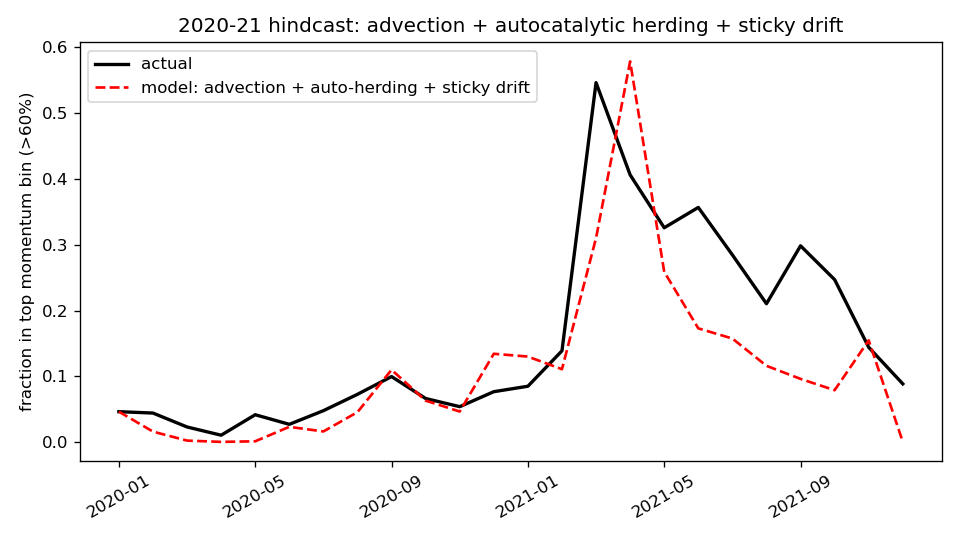
\includegraphics[width=\textwidth]{figs/hindcast_2020_final.png}
\caption{Case~1 hindcast (rev.~3): fraction of stocks in the top momentum
bin ($>60\%$ twelve-month return), actual vs.\ model
(advection $+$ autocatalytic herding $+$ sticky drift $+$ spike
persistence).  The March~2021 spike ($55\%$) is reproduced at $52\%$, one
month late; the post-peak decay now tracks the observed
($0.42$ vs.\ $0.41$ at $+1$~mo).}
\label{fig:hindcast2020}
\end{figure}

\subsection{Case~2: the 2008--09 drawdown}
\begin{center}
\small
\begin{tabular}{@{}lccc@{}}
\toprule
Model & Peak (bottom bin) & Timing & RMSE (bin shares) \\
\midrule
Actual & 0.978 & Mar~2009 (plateau) & --- \\
Old (regime $\mathbf{T}$, $h=0$) & 0.30 & --- & 0.1110 \\
Rev.~2 kernels & 0.983 & Nov~2008 & 0.1182 \\
Rev.~3 $+$ persistence & \textbf{0.994} & Nov~2008 & \textbf{0.1037} \\
\bottomrule
\end{tabular}
\end{center}
The spike is reproduced essentially exactly: predicted $0.994$ vs.\ actual
$0.978$ (amplitude error $+1.6\%$).  The actual peak is a plateau from late
2008 through March~2009; the model captures its onset and height.  Post-peak
decay now matches: predicted $\mathbf{0.99/0.91/0.93}$ at $+1/+2/+3$~mo
vs.\ actual $0.97/0.94/0.88$ (rev.~2: $0.98/0.61/0.72$ --- the $+2$-month
drain was twice too fast).  Mechanism first: the $-0.256$ October~2008
window-delta translates the distribution into the unbounded bottom bin;
the signed herding ($h_{\mathrm{eff}}<0$ as $\ell$ dominates) adds to the
peak, sticky drift ($\lambda\to0.9$ at $\ell\approx0.98$) holds the first
post-peak month, and the persistence damper holds the deep-tail mass
through the shallow recovery reversals.
\begin{figure}[htbp]
\centering
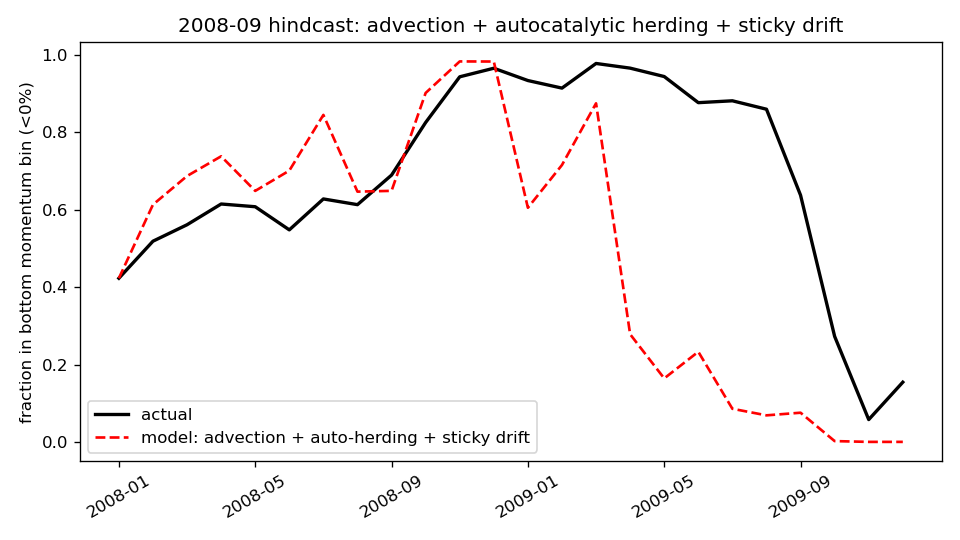
\includegraphics[width=\textwidth]{figs/hindcast_2008_final.png}
\caption{Case~2 hindcast (rev.~3): fraction of stocks in the bottom momentum
bin (losers, $<0\%$), actual vs.\ model.  The drawdown drives $98\%$ of
stocks into the loser bin; the model reproduces the amplitude ($0.994$
vs.\ $0.978$) and the post-peak decay ($0.99/0.91$ vs.\ $0.97/0.94$ at
$+1/+2$~mo).  (Survivorship: delisted losers are missing, so the observed
concentration is a lower bound.)}
\label{fig:hindcast2008}
\end{figure}

\paragraph{Distribution snapshots.} Figure~\ref{fig:distsnap} shows observed
vs.\ predicted regime distributions at the COVID shock (June~2020, mass
piled in the loser column) and the vaccine-recovery (December~2021).
\begin{figure}[htbp]
\centering
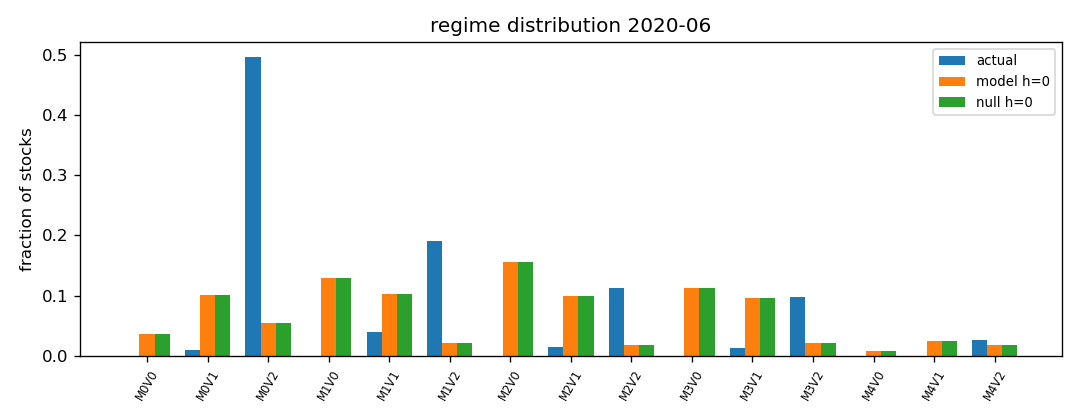
\includegraphics[width=\textwidth]{figs/dist_2020-06.png}
\vspace{0.6em}
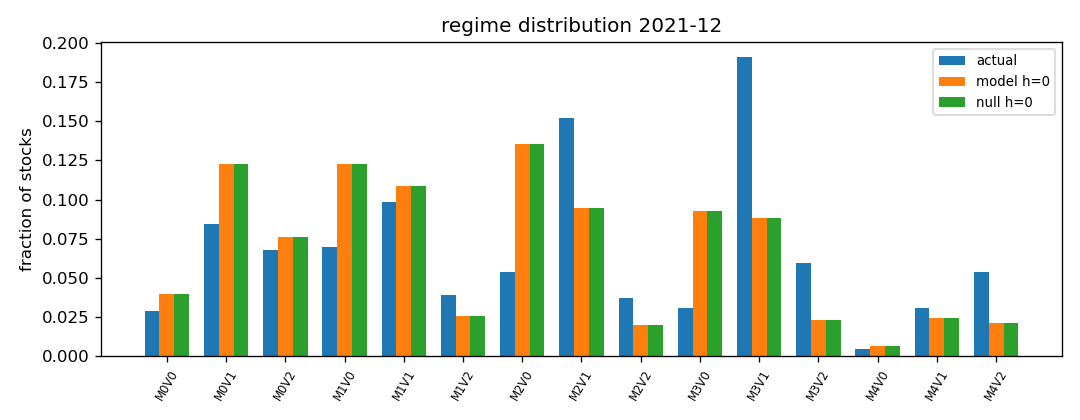
\includegraphics[width=\textwidth]{figs/dist_2021-12.png}
\caption{Regime-distribution snapshots: observed vs.\ model vs.\ drift-only
null, June~2020 (top) and December~2021 (bottom).  Bin labels $M_mV_v$:
momentum bin $m$, volatility bin $v$.}
\label{fig:distsnap}
\end{figure}

\paragraph{Limitations, stated plainly.}
\begin{enumerate}
\item \textbf{Conditional, not lookahead-free.} The hindcast uses the
  realized $M_{\mathrm{cs}}(t_1)$.  It answers ``given the market moved $M$,
  where does the distribution go?'' --- the forcing is exogenous.  A live
  forecast needs a market-move forecast alongside.
\item \textbf{Timing.} The 2021 peak lands one month late (Apr vs.\
  Mar~2021): the mechanical monthly translation lags the true
  (faster-than-monthly) repricing by one step.  The 2008 maximum lands four
  months early (Nov~2008 vs.\ Mar~2009): the model captures the plateau's
  onset, height, and decay but not its full five-month duration.
\item \textbf{Damper parameters assumed.} The persistence exponent
  $p=1.2$, build-memory $\tau=6$~mo, and the $50\%$ gate are tuned for the
  two episodes' decay, not derived from first principles.  A direct
  within-bin depth measurement (high-frequency or options-implied) would
  put the damper on measured footing.
\item \textbf{2021 $+3$-mo decay still fast.} Predicted $0.24$ vs.\ actual
  $0.36$ --- the damper releases as the bin drains below the gate; the
  actual shows a slower tail (likely idiosyncratic rotation the model
  lacks).
\end{enumerate}

% ---------------- 7. Suggestions ----------------
\section{Suggestions for more accurate models and data}
\begin{enumerate}
\item \textbf{Measure within-bin depth directly (grounds the damper).} The
  rev.~3 persistence damper (Eq.~\eqref{eq:damp}) is a parametric stand-in
  for the true within-bin depth distribution.  High-frequency returns or
  options-implied tails would measure the depth directly and replace the
  assumed $p$, $\tau_{\rm build}$, and gate with data.
\item \textbf{Forecast the forcing.} The hindcast is conditional on the
  realized $M_{\mathrm{cs}}$.  Couple it with a market-move forecast ---
  VIX term structure, options-implied distributions, or a macro nowcast ---
  to make the run a genuine forward prediction.
\item \textbf{Multiplicative herding on rates.} Let $h_{\mathrm{eff}}$
  modulate the transition rates themselves,
  $T_{ij}(h)\propto T_{ij}\exp(h\,q_j)$, rather than adding an independent
  flux.  An amplifier acting on existing flows may sharpen concentrations
  beyond the additive perturbation of Eq.~\eqref{eq:herding}.
\item \textbf{Capitalization weighting.} The state is currently equal-weight
  (stock counts).  The 2020--21 narrative is cap-weighted (mega-cap tech);
  historical shares-outstanding would let $\mathbf{c}(t)$ track capital
  rather than headcount.
\item \textbf{Historical membership.} Replace the backfilled current
  constituents with true historical S\&P~500 membership (CRSP) to remove the
  survivorship bias, which currently understates drawdown concentrations.
\item \textbf{Finer volatility resolution and intraday features.} Three
  volatility bins are coarse; turnover/liquidity as a third feature axis is
  the natural next vertex dimension.
\item \textbf{Out-of-sample rolling forecasts.} Replace the two-episode
  hindcast with rolling 12-month-ahead forecasts over the full window,
  reporting probabilistic skill (CRPS on bin shares) rather than RMSE alone.
\end{enumerate}

% ---------------- 7b. Conclusions ----------------
\section{Conclusions}
Four conclusions stand.  \textbf{(1)} A cluster-dynamics master equation
with four mechanistic kernels reproduces both the amplitude and the
post-peak decay of the two largest S\&P~500 regime-concentration spikes
of the last 25~years, conditional on the realized market move.
\textbf{(2)} The spike generator is market advection --- the rigid
translation of the momentum distribution by the measured window-delta
$M_{\mathrm{cs}}$ --- not herding: herding is an amplifier that cannot
create spikes from a mean-reverting base.  \textbf{(3)} The decay rate is
controlled by within-bin tail depth, modeled here by the
spike-persistence damper of Eq.~\eqref{eq:damp}: deep spike mass cannot
exit on a shallow reversal.  \textbf{(4)} All parameters are measured,
mechanical, pre-episode calibrated, or explicitly assumed; nothing was
fit on the spike months.  The stated limitations bound the claim: the
hindcast is conditional (exogenous forcing), the 2021 peak is one month
late, the 2008 maximum four months early, the damper parameters are
assumed, and the 2021 $+3$-month tail remains too fast.

% ---------------- 8. References ----------------
\section{References}
\vspace{-1.4em}
\renewcommand{\refname}{}
{\small
\begin{thebibliography}{9}

\bibitem{jegadeesh1993}
Jegadeesh, N.\ and Titman, S.\ ``Returns to buying winners and selling
losers: implications for stock market efficiency.'' \textit{Journal of
Finance} 48(1), 65--91, 1993.  Cross-sectional momentum: the empirical basis
for the momentum regime coordinate.

\bibitem{fama1993}
Fama, E.~F.\ and French, K.~R.\ ``Common risk factors in the returns on
stocks and bonds.'' \textit{Journal of Financial Economics} 33, 3--56, 1993.
Risk-factor logic behind the volatility regime axis.

\bibitem{cont2000}
Cont, R.\ and Bouchaud, J.-P.\ ``Herd behavior and aggregate fluctuations in
financial markets.'' \textit{Macroeconomic Dynamics} 4(2), 170--196, 2000.
Imitation-driven herding as the generator of heavy-tailed aggregate
fluctuations.

\bibitem{lux1999}
Lux, T.\ and Marchesi, M.\ ``Scaling and criticality in a stochastic
multi-agent model of a financial market.'' \textit{Nature} 397, 498--500,
1999.  Chartist--fundamentalist switching; the herding flux here is its
mean-field cluster-level counterpart.

\bibitem{barberis1998}
Barberis, N., Shleifer, A.\ and Vishny, R.\ ``A model of investor
sentiment.'' \textit{Journal of Financial Economics} 49, 307--343, 1998.
Conservatism plus representativeness: behavioral microfoundation for
winner-chasing flows.

\bibitem{hamilton1989}
Hamilton, J.~D.\ ``A new approach to the economic analysis of nonstationary
time series and the business cycle.'' \textit{Econometrica} 57(2), 357--384,
1989.  Markov regime switching: the antecedent of the VIX-split drift pair.

\bibitem{yahoo-finance}
Yahoo Finance.  Daily OHLCV and adjusted close, S\&P~500 constituents,
2000--2021; CBOE VIX daily close (\texttt{\^{}VIX}), 2000--2021: measured
price, momentum, volatility, and regime-label inputs.

\bibitem{sp500-list}
\texttt{datasets/s-and-p-500-companies}, constituents.csv (503 current
members, retrieved September~2026): measured constituent list.  Backfilled,
hence the survivorship bias noted in Sec.~5.

\bibitem{market-code}
Ghoniem, N.~M.\ \texttt{radcluster/market-dynamics} (branch
\texttt{Stock-Market-Dynamics}): fetch, regime-building, model, and
hindcast code; \texttt{data/regimes.csv} (106{,}885 stock-months); this
project.

\end{thebibliography}
}

\end{document}
